\documentclass{beamer}

\usepackage{caption}
\captionsetup[figure]{labelformat=empty}

\title{Exploratory analysis of Recurrent deforestation warnings in São Félix do 
Xingu - Brazilian Amazon}

\author{Alber Sanchez\\alber.ipia@inpe.br}
\institute{TreesLab\\Instituto Nacional de Pesquisas Espaciais\\Brazil}
\date{\today}

\begin{document}

\frame{\titlepage}

\begin{frame}
    \frametitle{Introduction}
    \begin{itemize}
        \item Deforestation by sucessive degradation remains an challenging 
            question in the scientitic literature.
        \item We think the potential answer to this question could lie in 
            DETER's warning data set.
        \item We use DETER data from 2016 to 2021 of São Félix de Xingu, Pará, 
            Brazil.
    \end{itemize}
\end{frame}

\begin{frame}
    \frametitle{DETER}
    \begin{itemize}
        \item TODO
    \end{itemize}
\end{frame}

% \begin{frame}
%     \frametitle{DETER}
%     \begin{figure}[h] 
%         \includegraphics[width=\linewidth]
%         {./figures/plot_deter_area_by_state_pyear_type.png}
%         \caption{DETER's total warning area by type, state \& PRODES year.}
%         \label{fig:deter_warnings_area_size}
%     \end{figure}
% \end{frame}

\begin{frame}
    \frametitle{Area of DETER warnings in SFX}
    \begin{figure}[h] 
        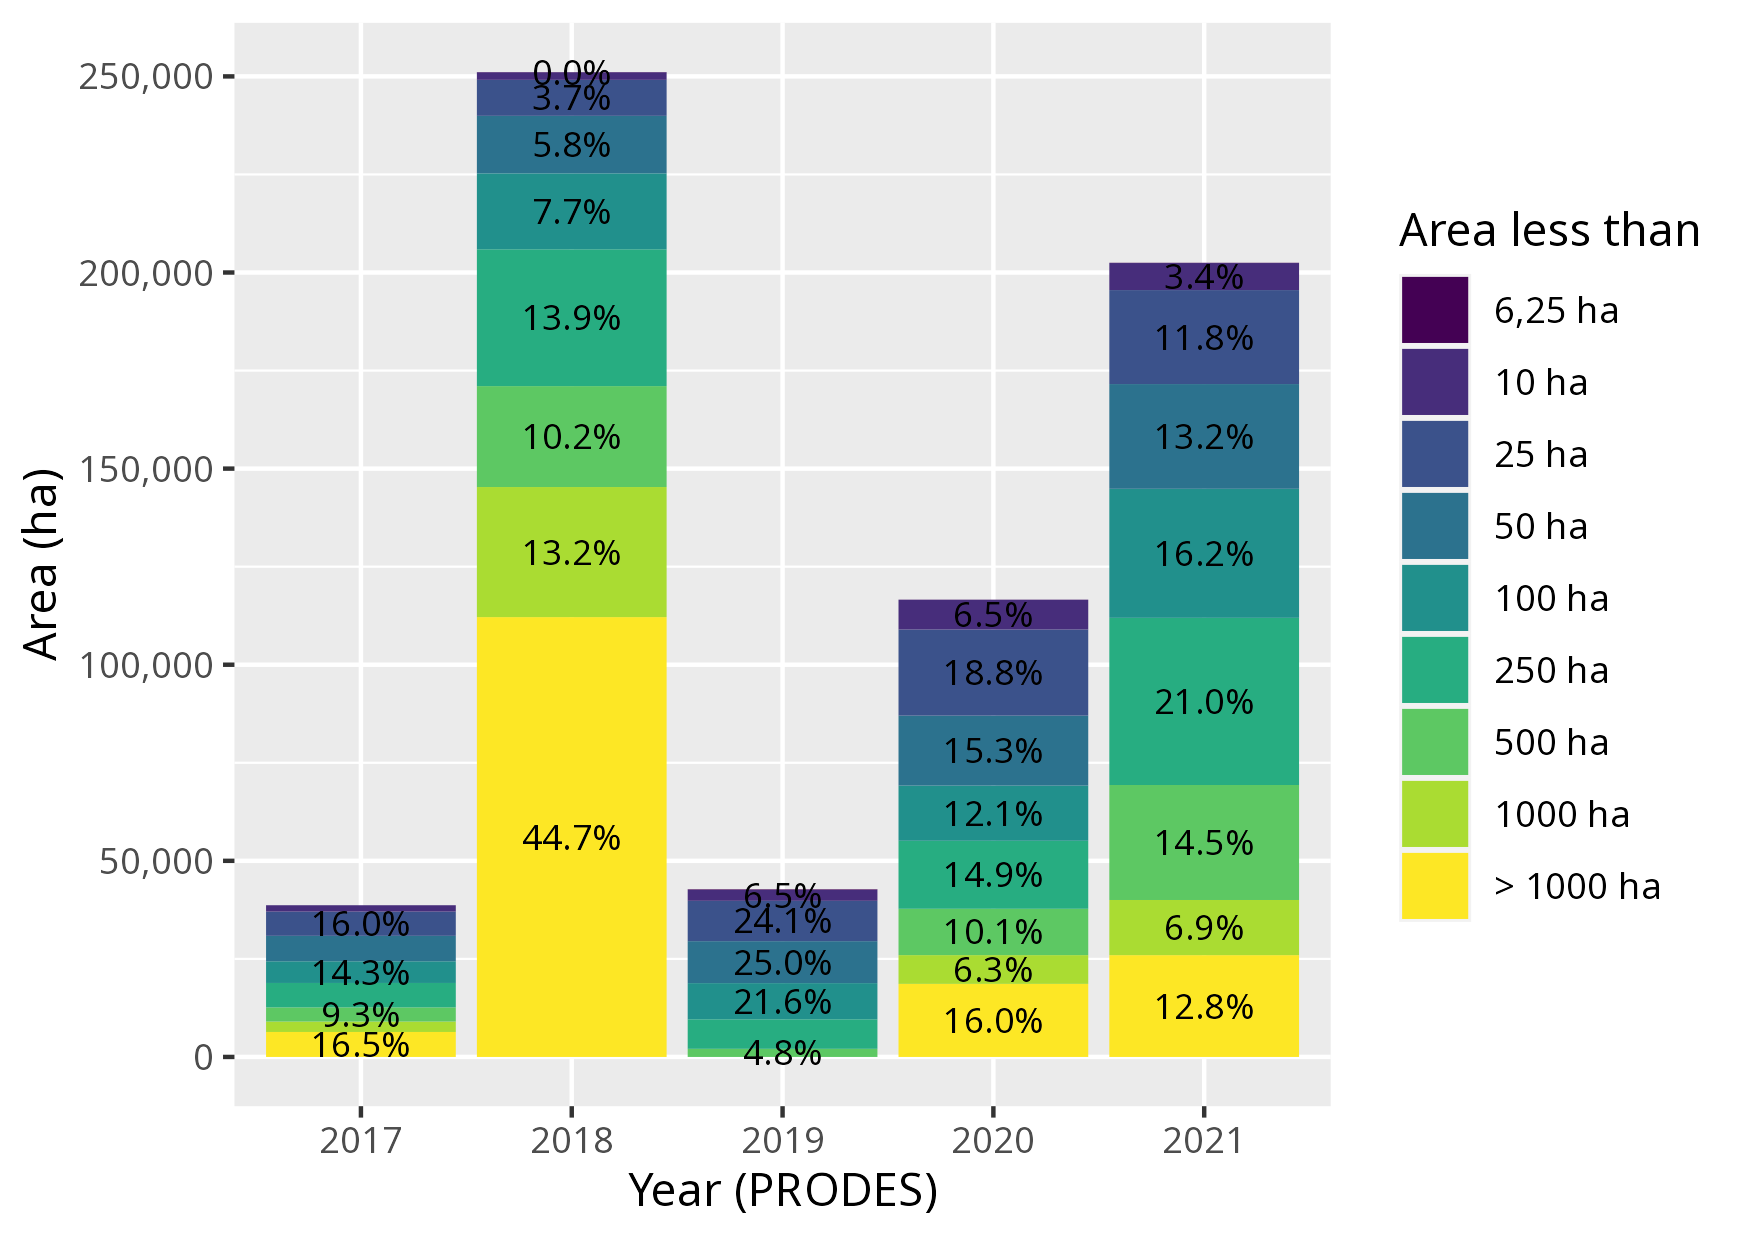
\includegraphics[width=\linewidth]
        {./figures_doc/deter_warnings_area_size.png}
        \caption{Note the increasing trend and its area distribution.}
        \label{fig:deter_warnings_area}
    \end{figure}
\end{frame}

\begin{frame}
    \frametitle{Number of DETER warnings in SFX}
    \begin{figure}[h] 
        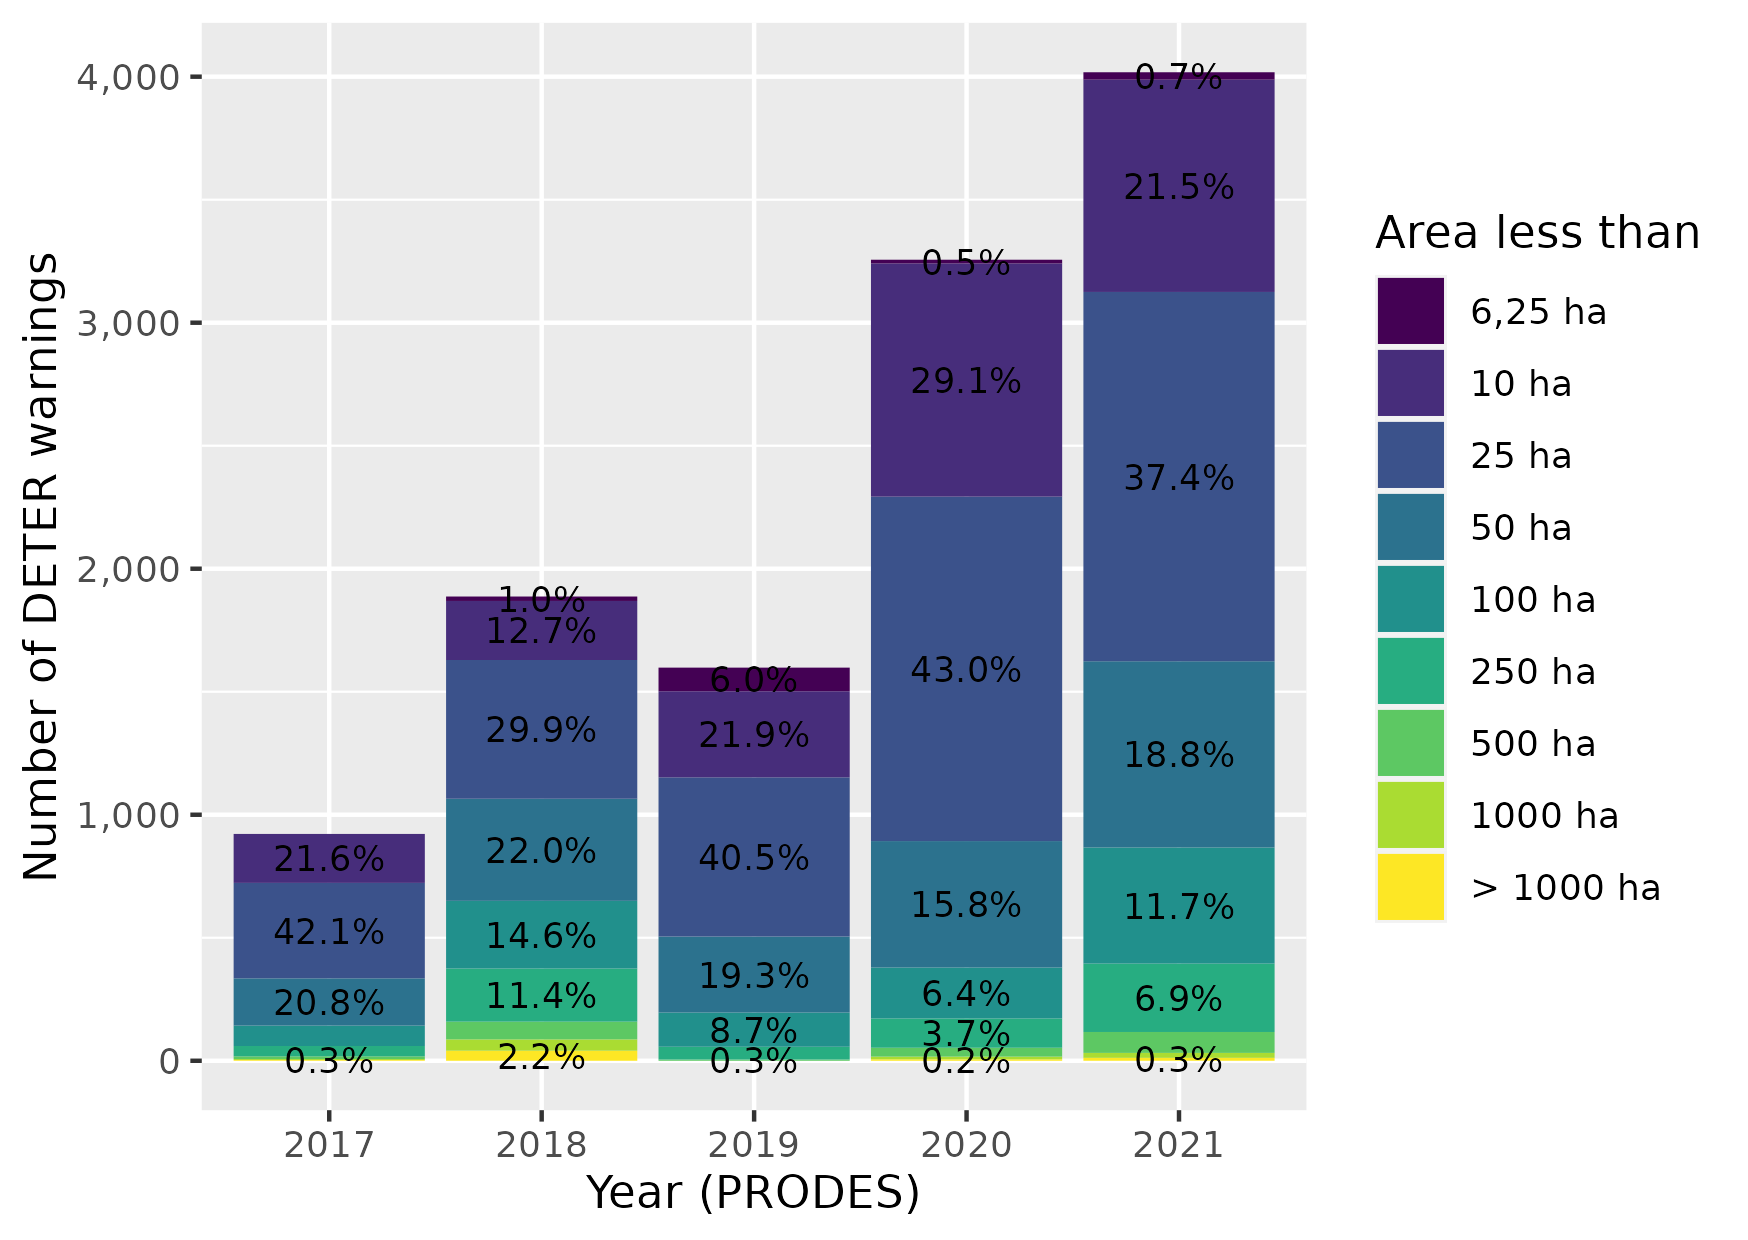
\includegraphics[width=\linewidth]
        {./figures_doc/deter_warnings_size.png}
        \caption{Note the increasing trend and the small peak in 2018.}
        \label{fig:deter_warnings_number}
    \end{figure}
\end{frame}

\begin{frame}
    \frametitle{Warning subareas}
    \begin{itemize}
        \item TODO: Explain what subareas are.
    \end{itemize}
\end{frame}

\begin{frame}
    \frametitle{Periodicity of DETER warnings in SFX}
    \begin{figure}[h] 
        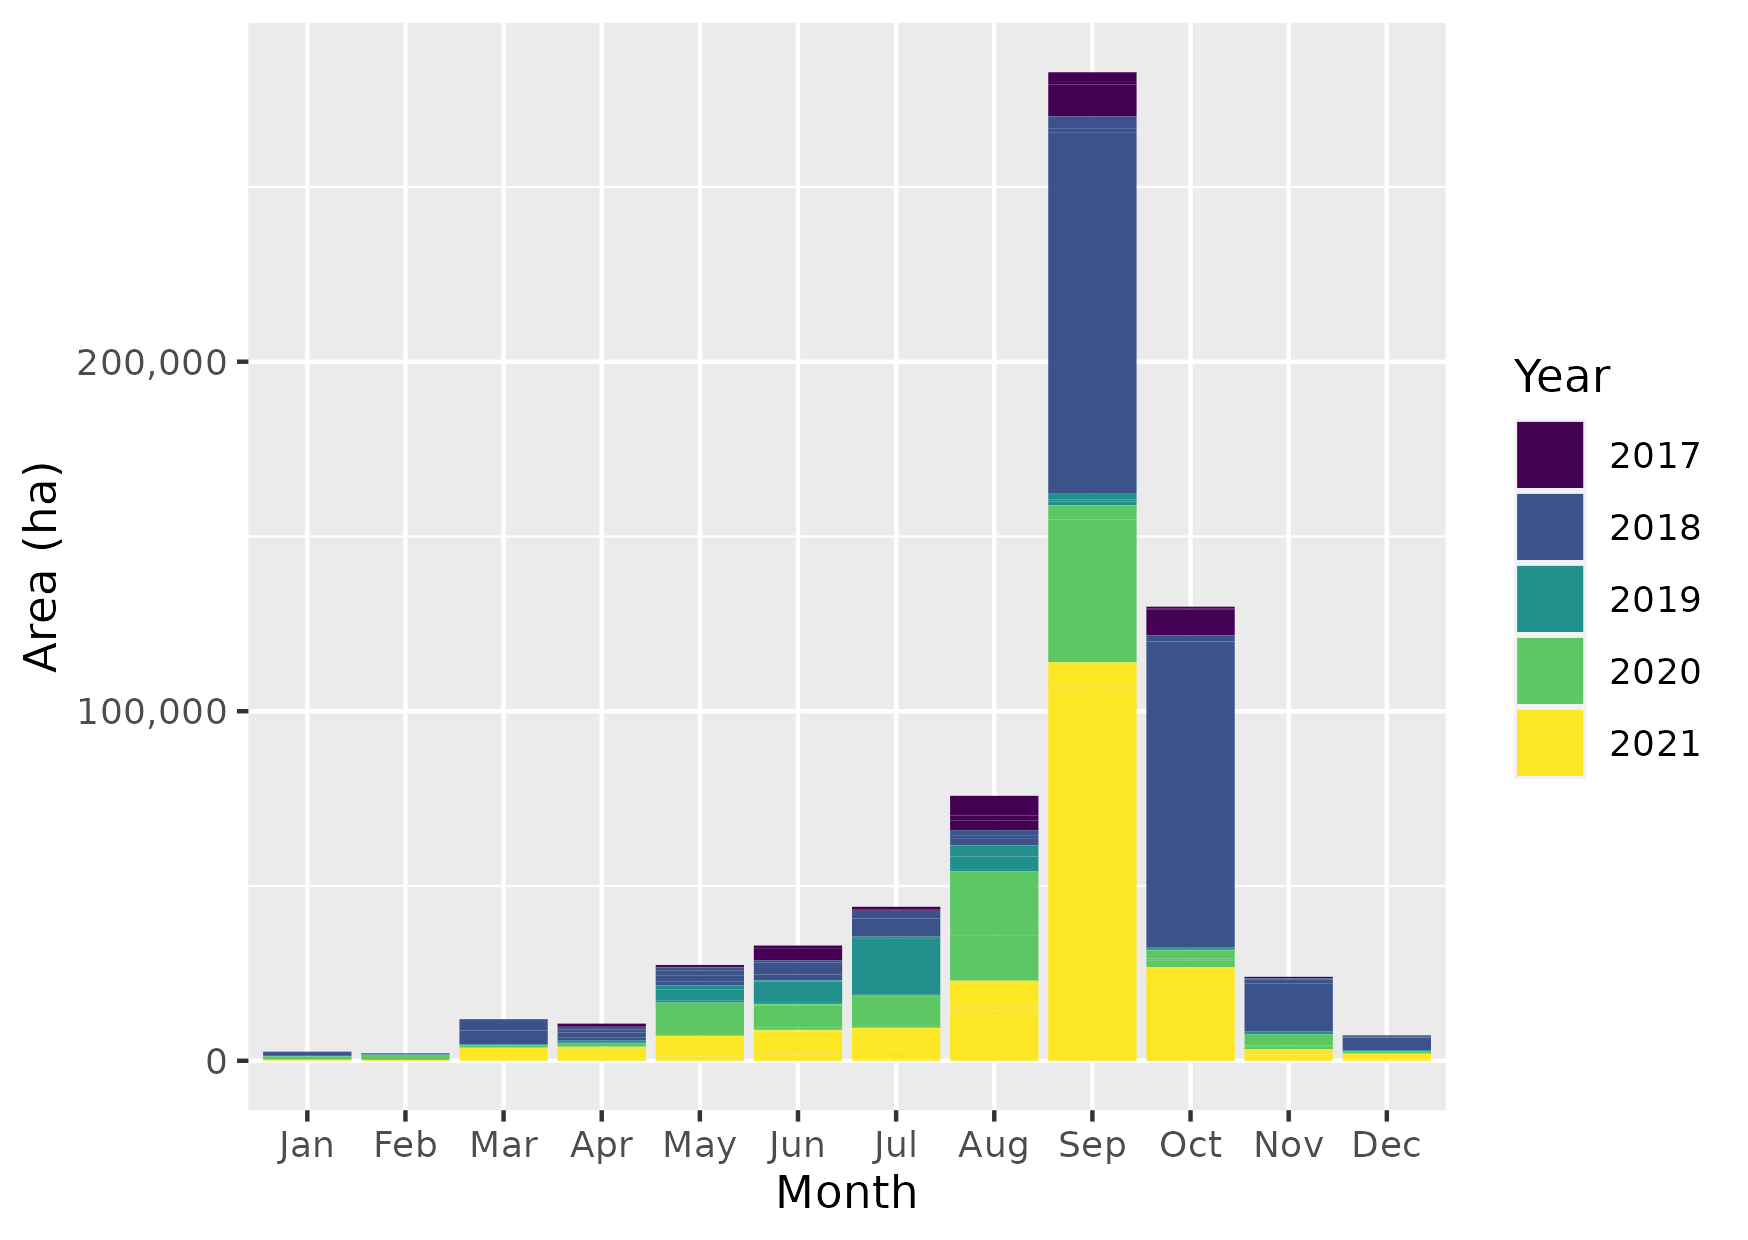
\includegraphics[width=\linewidth]
        {./figures_doc/deter_warnings_size_month.png}
        \caption{Note Sep-Oct 2018 and Aug-Sep 2020 }
        \label{fig:deter_warnings_periodicity}
    \end{figure}
\end{frame}

\begin{frame}
    \frametitle{Subareas of recurrent warnings}
    \begin{figure}[h] 
        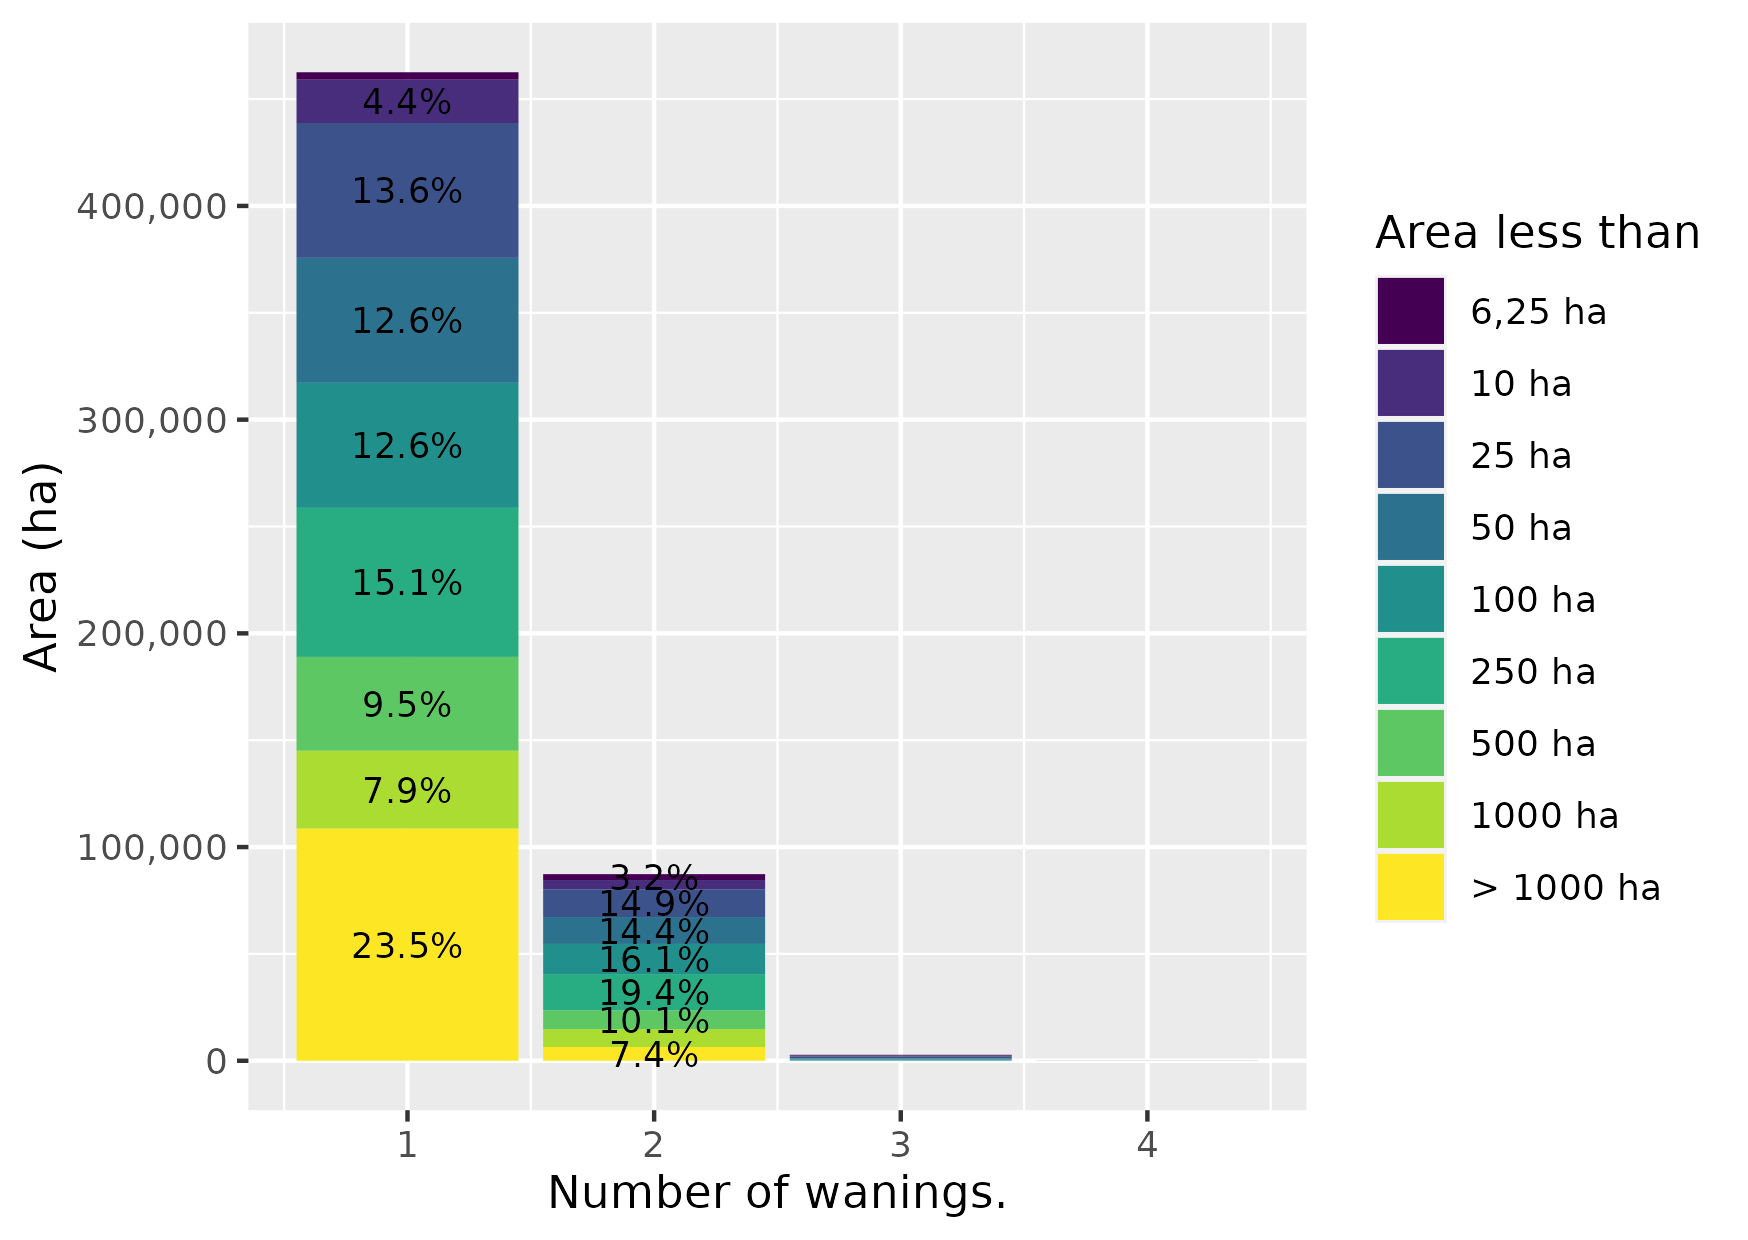
\includegraphics[width=\linewidth] 
        {./figures_doc/plot_area_by_warnings.png}
        \caption{Most subareas are issued a single warning.}
        \label{fig:deter_warning_recurrency}
    \end{figure}
\end{frame}

\begin{frame}
    \frametitle{Days between first and last warnings}
    \begin{figure}[h] 
        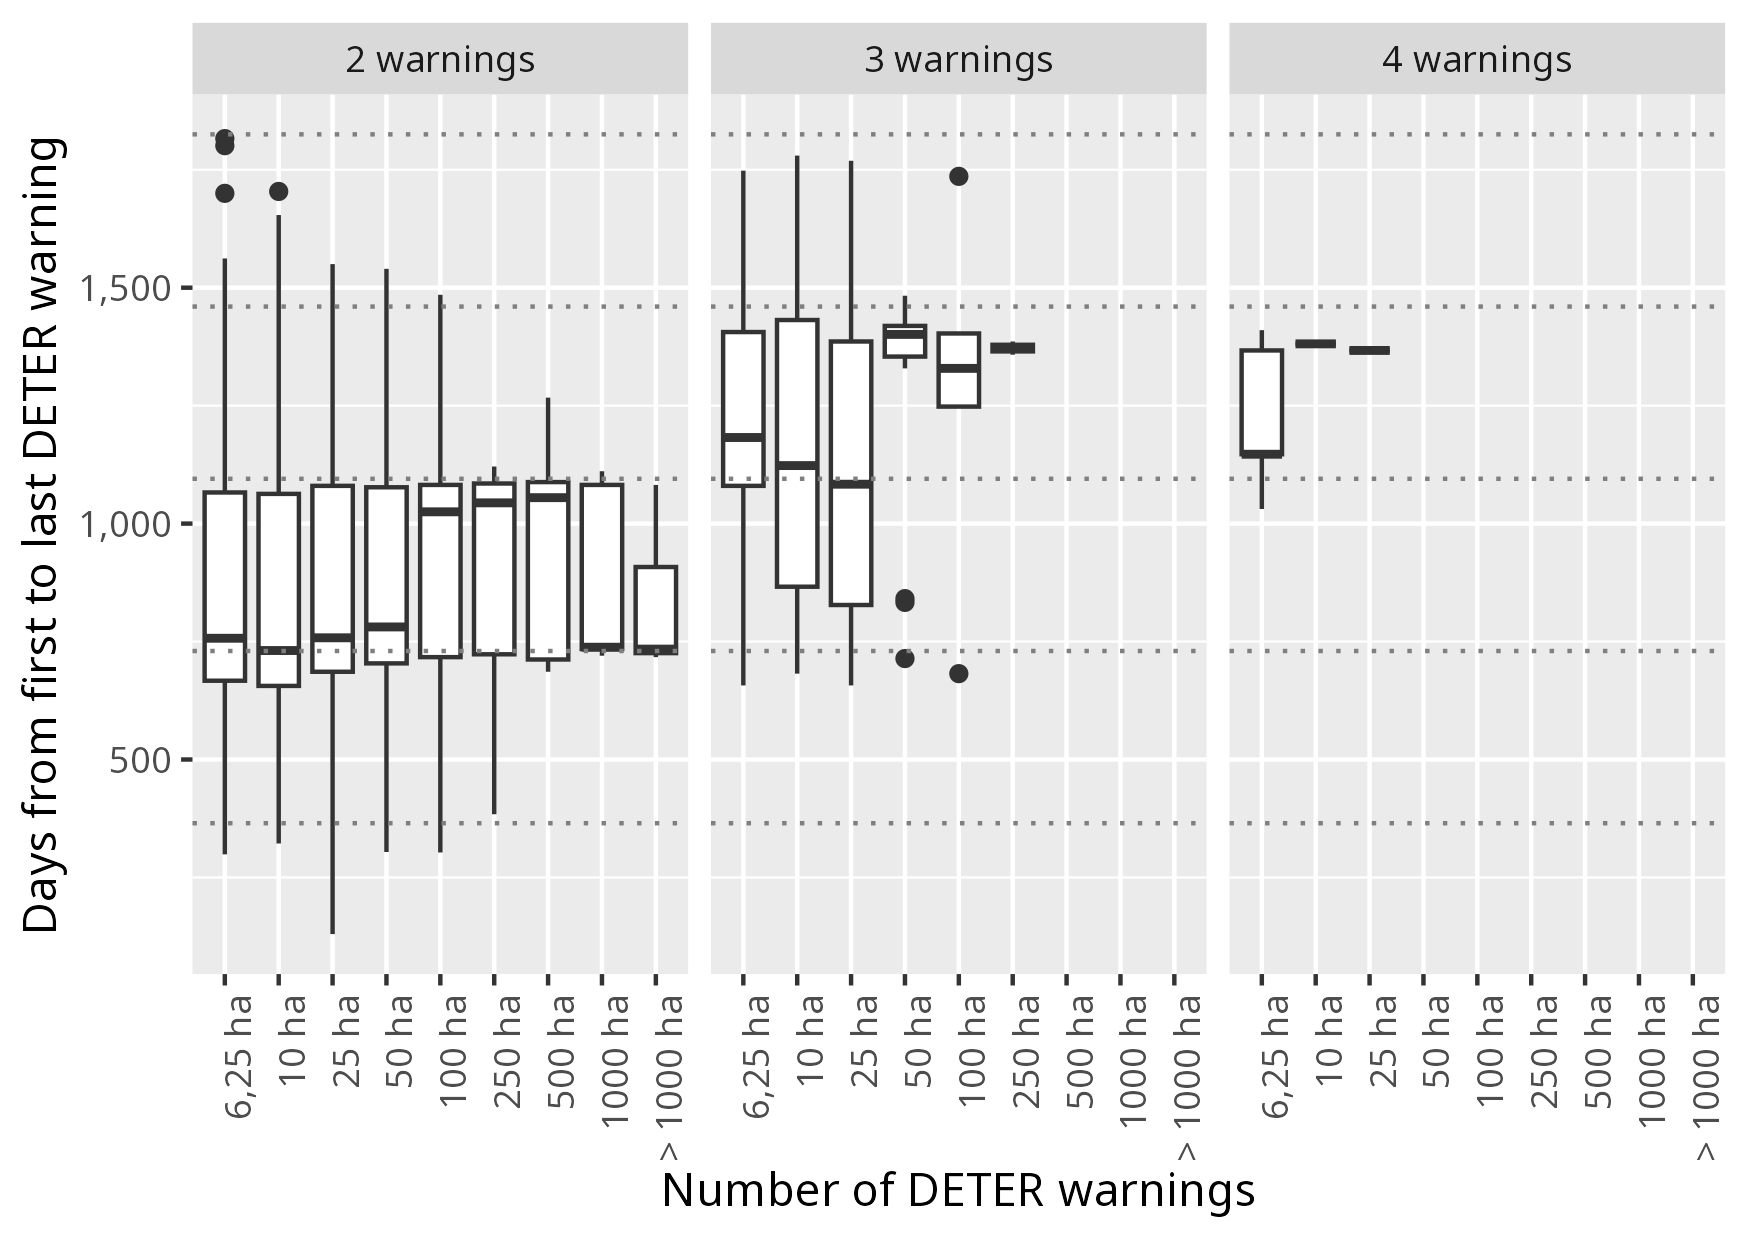
\includegraphics[width=\linewidth]
        {./figures_doc/plot_days_first_to_last.png}
        \caption{The mean lag between 2 and 3 warnings is one year.}
        % NOTE: Each Box plot shows the median; 
        %       the first and third quartiles (hinges); 
        %       1.5 times the inter-quartile range from the hinges; 
        %       and the outliers.
        \label{fig:deter_warning_first_to_last}
    \end{figure}
\end{frame}

\begin{frame}
    \frametitle{Discussion}
    \begin{itemize}
        \item Our results could help imporving the characterization of 
            degradation in the Brazilian Amazon.
        \item A potential application of our work is to identify 
            spatio-temporal areas which could help training Machine-Learning
            algorithms for automatic indentification of forest degradation.
    \end{itemize}
\end{frame}

\end{document}
